\chapter{Measurement Setup \& Techniques} \label{chapter:measurement}

In this chapter we discuss the measurement setup and techniques that we use in this thesis work. We present all individual parts of our signal generation and measurement chain, putting emphasis on the generation and measurement of high-frequency signals. Afterwards we briefly discuss the calibration and compensation techniques that we use to correct signal imperfections when generating qubit drive and flux signals. Finally we introduce the different measurement techniques that we use in this work, including qubit readout and driving as well as more advanced methods used to obtain all relevant qubit parameters such as frequency, anharmonicity as well as relaxation and dephasing times.

\smallskip

Our experimental setup consists of the qubit chip discussed in chapter \ref{chapter:design}, which is put at the 20 mK stage of a He$_3$/He$_4$ dilution cryostat and connected to a room temperature signal generation and measurement chain via cryogenic microwave components and 50 $\Omega$ coaxial transmission lines. At room temperature, we generate microwave pulses as well as DC and high-frequency flux bias pulses using heteordyne mixing and/or high-frequency arbitrary signal generators. We use a cryogenic amplifier chain and homodyne demodulation at room temperature to perform reflectometric measurements of the phase of our microwave readout signal.

\section{Sample Holder \& PCB}

\begin{SCfigure}[1][ht!]
	\centering
		\includegraphics[width=5cm]{"./material/photos/sample_holder"}
	\caption[]{The sample holder with the mounted PCB carrying the qubit chip. Bond wires are used to connect the on-chip tranmission lines to the PCB, which in turn uses a Mini-SMP connector to connect the bondwire to a set of external coaxial SMP cables. The top part of the sample holder is screwed to the bottom part, forming a closed box with cavities only for the tranmission lines and the qubit chip. The whole sample holder is screwed to the 20 mK stage of the dilution cryostat.}
	\label{fig:pcb_and_sample_holder}
\end{SCfigure}

For mounting the qubit chip as shown in fig. \ref{fig:} in the sample holder, it is first glued to a custom-designed high-frequency PCB, as shown in fig. \ref{fig:pcb_and_sample_holder} (bottom). On this PCB, six 50 $\Omega$ CPW waveguides terminated by Mini-SMP connectors are bond-wired to the drive/readout and fast flux lines of the qubit chip. For each qubit, one readout/drive line and two flux lines are present on the chip. In addition, bond wires are used to connect the ground plane of the chip to that of the PCB. On-chip bond wires are used to connect separated parts of the on-chip ground plane which are isolated from each other due to the circuit topology, which is important to avoid spurious on-chip resonances in the relevant frequency range $4-7$ GHz \citep{schuster_circuit_2007}. The PCB with the mounted chip is then screwed to a sample holder machined in copper that fully encloses the PCB, as shown in fig. \ref{fig:pcb_and_sample_holder} (top and bottom) and that consists of a bottom part on which the PCB is screwed and that is itself screwed to the top part of the sample holder. The top part provides holes for the SMP connectors and is pressed against the surface of the PCB. Machined grooves in the top part provide the necessary open space above the qubit chip and the transmission lines on the PCB. The function of the sample holder is to thermally anchor the PCB and the qubit chip to the cryostat and, more importantly, to shield the qubit chip from spurious electromagnetic signals and enclose it in a conducting cavity that is small enough to suppress box resonances at all relevant working frequencies.

\section{Signal Generation \& Acquisition}

\begin{figure}[ht!]
	\centering
		\includegraphics[width=1.\textwidth]{"./material/figures/2-qubit-processor/measurement setup"}
	\caption[The measurement setup used for the two-qubit experiments]{The measurement setup used for the two-qubit experiments. Exactly the same drive and readout scheme is used for both qubits with phase-locked microwave sources and arbitrary waveform generators.}
	\label{fig:measurement_setup}
\end{figure}

Fig. \ref{fig:measurement_setup} shows the wiring of our experiment from room temperature down to the 20 mK state of the dilution cryostat. Superconducting cables are used where adequate to minimize signal attenuation, in addition lossy cables made from special alloys such as CuNi are used to minimize heat transfer into the cryostat, which is especially critical between the 300 mK and 20 mK stages. Pairs of bifilar cables are used to provide DC biasing of one or several superconducting coils.

\subsection{Driving and Measurement of the Qubit}

Each of the qubits together with the corresponding readout resonator on our chip is fitted with an individual drive and readout circuit. At room temperature we generate qubit and resonator drive waveforms using phase-locked single-tone microwave sources whose continous output is mixed with fast control pulses generated by two arbitrary waveform generators (the details of this microwave mixing will be discussed in the following paragraph). The drive and readout signals are then combined and sent to the qubit chip through a series of (cryogenic) attenuators and filters. A cryogenic circulator at the 20 mK sample stage of the dilution cryostat routes the incoming pulses to the qubit chip where they are sent to the qubit readout resonator and finally reflected by it. The reflected signal passes again through the input microwave circulator and gets routed through a double isolator and a band-pass filter to a cryogenic HEMT amplifier with a gain of 40 dB. The amplified signal gets transmissted to the room temperature electronics, where it gets filtered and amplified further. Finally, the signal is demodulated with a continous microwave reference tone and fed to an ADC board through a pair of low-noise amplifiers.

\smallskip

In addition to this, each qubit is equipped with a pair of fast flux lines. High-frequency and DC flux pulses are generated using an arbitrary waveform generator at room temperature. The flux signal is then sent to the qubit chip through 20 dB of attenuation, a conventional Microtronics low-pass filter as well as a custom-made high-frequency powder filter that uses an absorptive material (Eccosorb) to attenuate high-frequency noise. After passing through the transmission line on the qubit chip, the outgoing flux signal gets routed to room temperature through a tranmission line identical to the input line. There, the signal can be measured, which is useful for correcting possible signal imperfections caused by the non-ideal character of the tranmsission line (we will detail in one of the following sections how to numerically compensate the imperfect frequency response of the flux line).

\subsection{Microwave Sideband Mixing}

To generate the qubit drive pulses we use single-sideband mixing techniques. We use a pair of IQ mixers that we drive with a continous single-frequency microwave tone and two synchronized fast control signals generated by an arbitrary waveform generator (Tektronix AWG5014b). In general, when feeding a signal $LO(t) = i_0 \cos{(\omega_{rf} t )}$ to the LO port of an IQ mixer and two signals $I(t)$, $Q(t)$ to the I and Q ports of the mixer, we obtain a signal

\begin{equation}
RF(t) = I(t)\cos{(\omega_{rf} t)}+Q(t)\sin{(\omega_{rf} t)} \label{eq:iqMixer}
\end{equation}

at the RF port of the mixer. Since the IQ mixer that we use is a passive, reciprocal device one can as well feed two input signals to the LO and RF ports and obtain the demodulated signal quadratures at the I and Q ports, a technique that we make use in our qubit readout scheme, as will be detailed later in this chapter.

Typically we use sideband mixing to generate drive pulses that are displaced in frequency in respect to the original LO (carrier) waveform. This if often advantageous since it eliminates microwave leakage at the signal frequency for zero voltage on the IQ inputs, which is often a big problem for commercially available IQ mixer, as we will discuss below.

\begin{figure}[ht!]
	\centering
		\includegraphics[width=0.7\textwidth]{"./material/figures/measurement/mixer_imperfections"}
	\caption[...]{Illustration of the method used to measure and correct the imperfect signal behavior of the IQ mixer used in our experiments: To minimize the leakage of the LO signal to the RF port, we apply a continous input signal at frequency $\omega_{rf}$ to the LO port and minimize the power at $\omega_{rf}$ the RF port by tuning the two offset voltages $I_0$ and $Q_0$ at the IF1/I and IF2/Q ports. To correct phase and amplitude errors during heterodyne mixing, we apply the same signal as before to the LO port and in addition two sideband signals to the IF ports. We then minimize the measured power at the RF port at $\omega_{rf}+\omega_{IF}$ by adding a correction waveform the IF ports.}
	\label{fig:iq_mixer_correction}
\end{figure}

Commercially available IQ mixers often deviate from the ideal behavior as given by eq. (\ref{eq:iqMixer}). Typical imperfections include large insertion losses --i.e. loss of signal power between the different ports of the mixer--, RF signal leakage at zero IQ-input and frequency-dependent phase and amplitude errors of the mixed sideband signals. In order to achieve reliable single-qubit operations we need to correct the signal leakage and quadrature-specific amplitude and phase errors. The signal leakage causes a small part of the LO signal to leak through to the RF port even when the IQ inputs are zeroed. This leakage can be compensated by adding center-frequency $\omega_c$ dependent DC offset voltages to the IQ ports. The appropriate offset voltages can be determined by applying a continuous input signal at a frequency $\omega_c$ to the LO port of the mixer and minimizing the measured signal power at the RF port by varying the IQ offset voltages. To correct the sideband amplitude and phase errors we apply another correction procedure that we outline here. First, for the signals at the IQ inputs of the mixer we introduce the notation

\begin{equation}
A(t) = I(t)+iQ(t) = a(t)\exp{(-i\phi(t))} \label{eq:iq_if_input}
\end{equation}

We consider an IQ signal at a single sideband frequency $\omega_{IF}$ and at fixed complex amplitude $a(t) = a = a_0\exp{(i\phi_0)}$ such that $A(t) = a\exp{(-i \omega_{IF} t)}$. The effect of the gain and phase imperfections of the IQ mixers can then be modeled by assuming that the mixer adds another IQ signal $\epsilon(\omega_{IF},\omega_{RF})A^*(t)$ at the mirrored sideband frequency $-\omega_{IF}$. We can correct this unwanted signal by adding a small correction $c(\omega_{IF},\omega_{RF})A^*(t)$ to our IQ input signal. The complex-valued correction coefficient $c(\omega_{IF},\omega_{RF})=|c|\exp{(i\angle c)}$ usually depends both on the carrier frequency $\omega_{RF}$ and the sideband frequency $\omega_{IF}$. We determine the correction coefficients by generating a continuous waveform at a given center and sideband frequency, measuring the amplitude of the unwanted sideband signal with a fast spectrum analyzer and minimizing its amplitude by varying the correction coefficient $c(\omega_{IF},\omega_{RF})$.

Both the offset and the sideband-amplitude and -phase corrections have been automated using our data acquisition software. By using the optimization techniques described above we can achieve $\le-80\;\mathrm{dBm}$ residual leakage power at the RF port of the mixer when no input IQ signal is present and a supression of the unwanted mirror sideband during heterodyne modulation by $>70\;\mathrm{dB}$.

\subsection{Fast Magnetic Flux Pulses}

We use a pair of superconducting coaxial cables to realize the qubit flux lines. Each qubit is connected to an on-chip transmission line, whose ends are connected to two fully symmetric transmission lines through the PCB. These two lines lead back to the room-temperature stage and can be used to send signals down the flux line and measure the transmitted signal. Between room temperature and the 20 mK stage of the cryostat, we apply 20 dB attenuation to each line and low-pass filter all signals both at the 4K and 20 mK stages of the cryostat. The low-pass filters at the 20 mK stage consist of custom-built powder filters made from a commercially available, highly absorptive and lossy material (Eccosorb, \citep{}). Appendix \ref{} contains details on the fabrication and frequency attenuation characteristic of these filters. The heavy filtering of the flux line is necessary since it reduces the high-frequency noise seen by the qubit. On the other hand, it also distorts all deterministic input signals that we send through the flux line, which is an unwanted effect and has to be corrected. For this, we measure and compensate the frequency response of the flux line by sending a well-defined test signal down the line and measuring the transmitted signal at the other end of the line. This allows us to obtain the response function of the input line. Fig. \ref{fig:FluxLineResponseFunction}a shows the model of the qubit flux line that we use to model the response function of the line. We assume that the response of the line is given by

\begin{figure}[ht!]
	\begin{center} 
	\begin{tabular}{c}
	 \includegraphics[width=0.5\textwidth]{"./material/figures/measurement/fluxline_model"} \\
	 \includegraphics[width=0.6\textwidth]{"./data/ct5/2011_04_04 - flux tomography/flux tomography"}
	 \end{tabular}
	\end{center}
	 \caption[]{(response function filtered with a Gaussian filter with a cut-off at 0.4 GHz)}
	 \label{fig:FluxLineResponseFunction}
\end{figure}

%
\begin{equation}
\chi_{\mathrm{fl}}(\omega) = \chi_{signal}(\omega)\cdot \chi_{DAC}\cdot \chi_{\mathrm{input}} \cdot \chi_{\mathrm{output}}\cdot\chi_{ADC} \label{eq:flux_response}
\end{equation}
%
Here, $\chi_{\mathrm{signal}}$ is the Fourier transform of the ideal input signal, $\chi_{ADC}$ and $\chi_{DAC}$ describe the response functions of the DAC and ADC, $\chi_{\mathrm{input}}$ and $\chi_{\mathrm{output}}$ corresponds to the response function of the input and output transmission lines. We can assume that $\chi_{\mathrm{input}}\approx\chi_{\mathrm{output}}$ since the input and output lines are symmetrical. By measuring $\chi_{\mathrm{fl}}$ and correcting the measured Fourier spectrum for the response function of the ADC $\chi_{ADC}$ (which can be measured separately) we obtain the input line response $\chi_{DAC}\chi_{\mathrm{input}}$ including the DAC response that we can then correct by applying
%
\begin{equation}
\chi_{\mathrm{signal}}^{\mathrm{corr}} = \chi_{\mathrm{signal}}\cdot (\chi_{DAC}\cdot\chi_{\mathrm{input}})^{-1}\cdot \mathrm{G}(f_0).
\end{equation}
%
Here, $G(f_0)$ is a Gaussian filter function that we apply to the measured response function to renormalize the signal distortion at high frequencies that is caused by the fact that we are not able to accurately measure the response function of the flux line above a certain frequency treshold due to the limited bandwidth of our measurement equipment. Usually, we set this cutoff frequency to $f_0=300\;\mathrm{MHz}$ which allows us to correct most signal distortion in the frequency band up to $f=1\;\mathrm{GHz}$ that is relevant to this work.

\smallskip

After having corrected the response of the flux line by this technique, we can further reduce signal distortion by directly probing the flux seen by the qubit at a given time by measuring the qubit frequency as a function of the time while applying a flux test signal to it. The measurement of the qubit frequency is done by driving it with a calibrated $X_\pi$ Rabi pulse and maximizing the measured $\ket{1}$ occupation probability after the pulse by tuning the qubit drive frequency. Using this technique, we can achieve a time resolution that is comparable to the length of the Rabi pulse that we use and which, for this work, is about $3-4\;\mathrm{ns}$. After having reconstructed the flux signal seen by the qubit, we can calculate the response function of the flux line and again correct it by changing the input signal. Fig. \ref{fig:FluxLineResponseFunction}b shows the measured flux signal seen by the qubit, the corresponding response function and the corrected input waveform for one of our qubits.

\subsection{Pulse Synchronization}

In our experiment, each qubit possesses two microwave sources that generate the drive and readout signals for it. The fast drive pulses for each qubit are generated by a single arbitrary waveform generator (AWG). A second AWG generates the flux pulses for the two qubits. The measurement of the reflected and demodulated readout signal of both qubits is done by a single ADC card. All these different signal generators and measurement devices need to be synchronized in order to maintain the relative phases and time differences between them between individual runs of our experiment. For this, we use a 10 MHz frequency reference chain, whose master clock is generated by the AWG that is responsible for generating the qubit drive pulses. The reference signal is then passed on to all microwave sources and signal generators as well as oscilloscopes, spectrum analyzers and ADC cards in our setup. In addition, to avoid random phase-jitter between the signals of the two microwave sources that generate the drive pulses of the two qubits, their drive frequencies need to be chosen such that they correspond a multiple of the repetition frequency of the master AWG, which is typically 50 kHz. If this condition is met, the relative phases between the two microwave signals is conserved between individual runs of the experiment, which is crucial when performing measurements that are sensitive to this phase such as quantum state tomography of entangled two-qubit states. In addition, a 1 GHz phase synchronization chain is used to phase-lock the two microwave generators and reduce phase drift between them.

\section{Measurement Techniques}

In this section, we discuss the techniques used to characterize and manipulate our two-qubit processor. We will cover the qubit readout and manipulation and will describe how we can determine all relevant qubit parameters using microwave reflectometry measurements.

\section{Qubit Readout}

\begin{figure}[ht!]
\centering
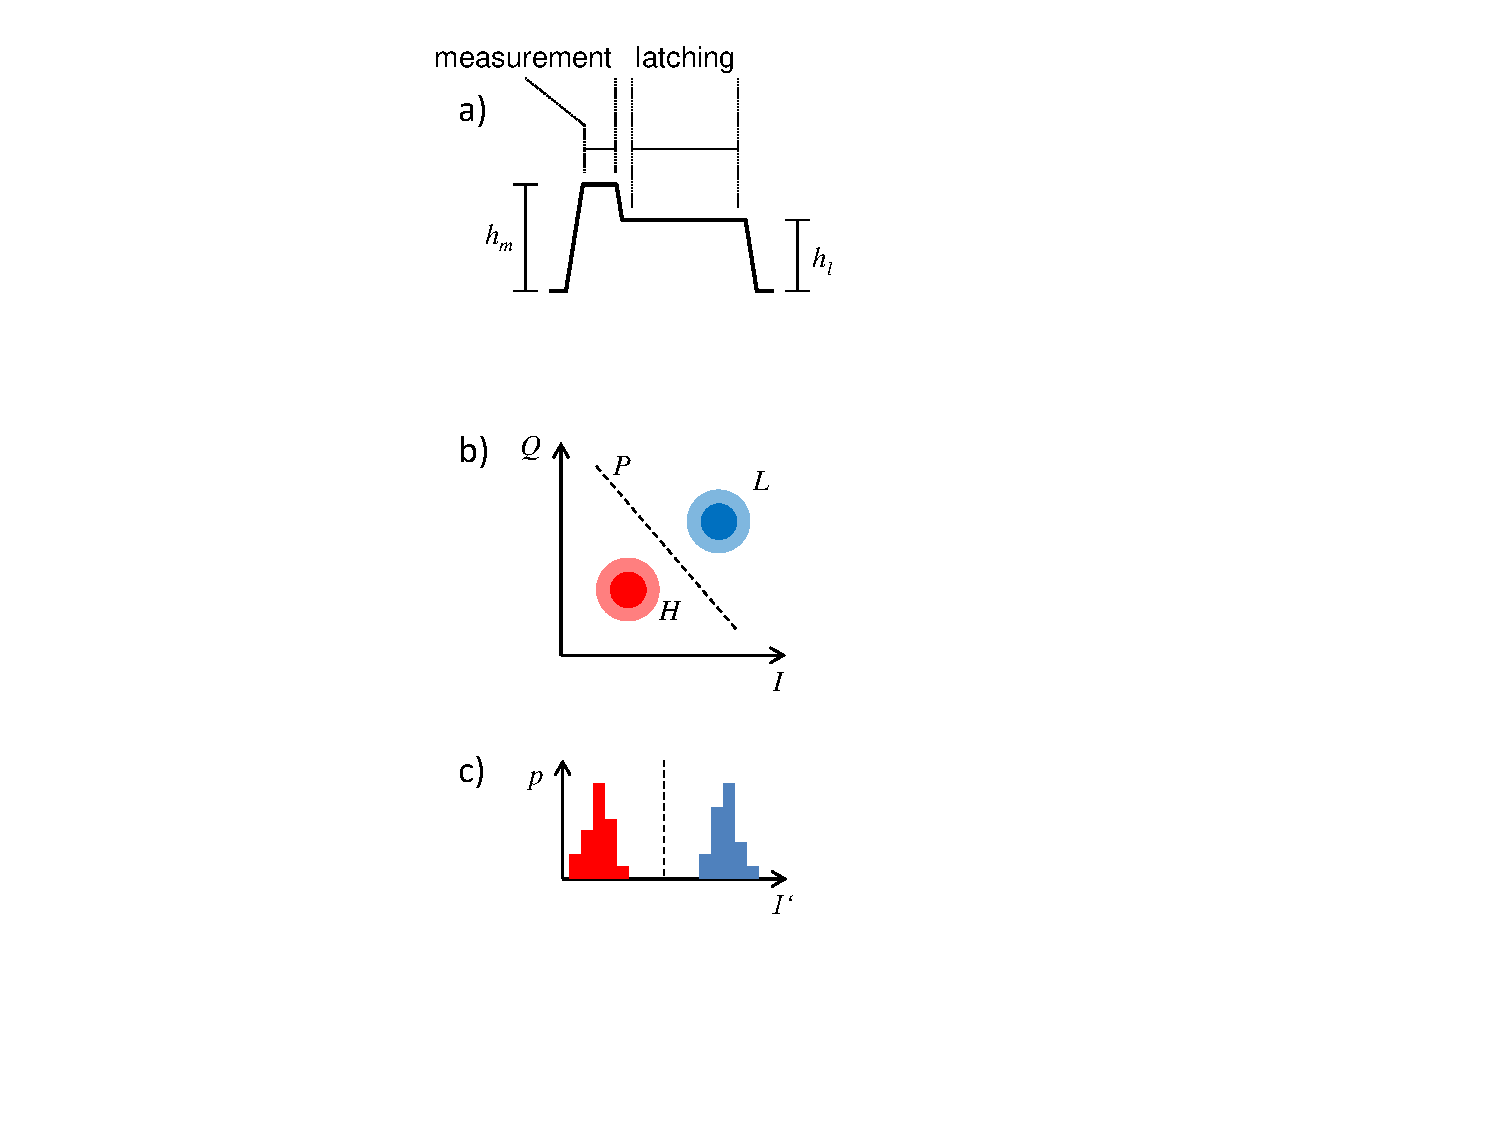
\includegraphics[width=\textwidth]{./material/figures/measurement/readout}
\caption{...}
\label{fig:readout_bringup}
\end{figure}

The general readout principle of the CJBA readout that we use in this work is described in section \ref{section:cjba}. Here we explain how we choose the frequency and drive amplitude working point for the readout. For all measurements described in this paragraph, the qubit is assumed to be in the $\ket{0}$ state all the time. To bring up the readout, we first determine the resonance frequency $f_r$ of the CJBA by reflectometry. We then choose a relative drive detuning $\Omega>\sqrt{3}$ at which the bistable regime is accessible. We mix the continous drive signal with a drive pulse as shown in fig. \ref{fig:readout_bringup}a. We attenuate the resulting drive signal using a tunable attenuator at room temperature and send it to the sample. The reflected and amplified signal is then demodulated with the continous input drive signal using an IQ demodulator. The resulting I/Q quadrature signals get then again amplified and digitized by an ADC card at a sample rate of 1 GHz, where we measure the signal only in the time window $t_m$ indicated in fig. \ref{fig:readout_bringup}a. We average the digitized I/Q signals over the whole measurement window to obtain a single measurement point in the IQ plane and repeat this sequence a large number of times (typically $10^4$). We repeat this sequence while ramping the attenuation, each time calculating the variance $\sigma_{IQ}^2=\mathrm{var}(Q)+\mathrm{var}(I)$ of the obtained set of points. When reducing the attenuation, at some point the input power sent to the CJBA will be sufficient to make it switch from the L to the H state, thereby changing the phase and consequently the I/Q values of the obtained signal. $\sigma_{IQ}^2$ will be biggest at a power where approximately 50 \% of switching occurs, as shown in fig. \ref{fig:readout_bringup}b. By substracting the average (I,Q) values at this point and performing a principal axis transformation that diagonalizes the covariance matrix
%
\begin{equation}
\mathrm{var}_{IQ} = \left(\begin{array}{cc}\mathrm{var}(I) & \mathrm{cov}(I,Q) \\ \mathrm{cov}(I,Q) & \mathrm{var}(Q) \end{array}\right).
\end{equation}
%
We can project the measured (I,Q) data points on the axis P in fig. \ref{fig:readout_bringup} and obtain a 1D probability distribution. The obtained offsets $I_0$, $Q_0$ and principal axis rotation angle $\alpha_{IQ}$ gives us then the discrimination criterion $Q_L<Q_0+\tan{\alpha_{IQ}}(I-I_0)$ that we use to classify new data points as belonging either to a L or H state. If measurement window is large enough and no retrapping occurs during the meausurement, the distributions corresponding to the L and H states will not overlap, yielding perfect discrimination between them.

\smallskip

After having determined the $I_0$, $Q_0$ and $\alpha_{IQ}$ we tune the attenuation such that we obtain $\approx 20\%$ switching, which usually gives us sufficient readout contrast to perform a qubit spectroscopy, as described in section \ref{section:qubit_spectroscopy} and calibrate a $X_\pi$ Rabi pulse, as described in section \ref{section:qubit_rabi}. We can then measure the switching probability of the CJBA readout as a function of the input power for the qubit in the state $\ket{0}$ and $\ket{1}$. Fig. \ref{fig:s_curves_example} shows an example of such an s-curve measurement. The difference between the two curves corresponding to the $\ket{1}$ and $\ket{0}$ corresponds to the readout contrast and allows us to choose the optimum drive power that yields the highest readout contrast. If desired, we can also perform a $X_\pi^{12}$ pulse on the qubit to put it in the state $\ket{2}$. In this state, the dispersive shift of the resonator frequency is larger than in the state $\ket{1}$, usually yielding a comparatively higher readout contrast, as shown in fig. \ref{fig:s_curves_example}. This is advantageous when performing e.g. single-run quantum algorithms on the processor, as described in chapter \ref{chapter:grover_algorithm}.

\section{Qubit Manipulation}

To drive the qubits, we need to generate fast microwave pulses with a well defined frequency and phase. As described in one of the previous paragraphs we can use IQ sideband mixing to shape arbitrary drive pulses of the form
%
\begin{equation}
u(t) = I(t)\cos{\omega_{rf}t}+Q(t)\sin{\omega_{rf}t}
\end{equation}
%
We can rewrite this as a product of two complex quantities
%
\begin{equation}
u(t) = \Re\left[ A(t)\cdot\exp{\left(-i\omega_{rf} t\right)}\right]
\end{equation}
%
where we defined, as before, $A(t)=I(t)+iQ(t)$. The reference phase defining an x-pulse can be chosen arbitrarily but must be conserved during one single experimental run. Thus, to realize a rotation of the qubit state in the xy-plane of the bloch sphere around an axis defined through an angle $\phi$ we can use a Gaussian-shaped pulse of the form
%
\begin{equation}
A(t) = A_0\cdot\exp{\left(-\frac{(t-t_0)^2}{2\sigma_t}\right)}\cdot\exp{\left(-i\phi\right)}
\end{equation}
%
In the following chapter we will discuss more in detail the calibration of these drive pulses and possible errors induced when driving the qubit at frequencies comparable to its anharmonicity. 

\subsection{Spectroscopic Measurements of the Qubit State}

\begin{figure}[ht!]
\centering
\includegraphics[width=0.49\textwidth]{"./material/figures/measurement/qubit_spectroscopy"}
\includegraphics[width=0.49\textwidth]{"./data/ct5/2011_04_21 - grover and tomo/example - qubit 2 spectroscopy"}
\caption[]{Example of a measured qubit spectroscopy. Shown is the switching probability of the qubit readout when driving the qubit with a very long drive pulse (typically 1 $\mu$s) at a given drive frequency. The resonance to the right corresponds to the $\ket{0}\to\ket{1}$ (at frequency $f_{01}$)transition of the qubit, the resonance on the left to the 2-photon $\ket{0}\to\ket{2}$ (at frequency $f_{02}/2$) transition. We perform a Lorentzian fit of the two resonances to obtain the $\ket{0}\to\ket{1}$ and $\ket{0}\to\ket{2}/2$ resonance frequencies, from which we can calculate all other qubit transition frequencies.}
\label{fig:qubit_spectroscopy_example}
\end{figure}

In order to characterize the transition frequency and anharmonicity of the qubit it is useful to perform spectroscopic measurements of the qubit state. For this we drive the qubit with a very long Rabi pulse (usually $> 500\;\mathrm{ns}$ at a well-defined frequency $f_r$. When the drive frequency $f_r$ corresponds to the $f_{01}$ frequency of the qubit the drive pulse will induce a strong Rabi oscillation of the quantum state of the qubit. Since the decoherence time of the qubit is of the order of the length of the drive pulse, the qubit state will decay and dephase during the driven evolution, effectively yielding an equal probability to measure the qubit in either of the states $\ket{0}$ or $\ket{1}$ at the end. When the drive frequency is detuned from the qubit transition frequency, no oscillation will be induced and hence the qubit will remain in the state $\ket{0}$. The width of the resonance in frequency space is inversely proportional to the dephasing time of the qubit, following the equation
%
\begin{equation}
...
\end{equation}
%
Fig. \ref{fig:qubit_spectroscopy_example} shown an exemplatory qubit spectroscopy. Plotted is the probability of measuring the qubit in state $\ket{1}$ after applying a $1\;\mathrm{\mu s}$ rabi pulse at a given drive frequency to it. The blue curve has been measured at $10\;\mathrm{dB}$ higher power than the red curve and shows the $\ket{0}\to\ket{2}$ transition of the qubit. By fitting the resonance curves with a Lorentzian model we obtain the qubit frequencies $f_{01}$ and $f_{02}/2$, which allow us to calculate the effective Josephson and charging energies at the given working point.

\subsection{Rabi Oscillations}

\begin{figure}[ht!]
\centering
\includegraphics[width=0.49\textwidth]{"./material/figures/measurement/qubit_rabi_oscillation"}
\includegraphics[width=0.49\textwidth]{"./data/ct5/2011_04_21 - grover and tomo/example - qubit 2 rabi"}
\caption[]{Example of a measured qubit Rabi experiment. Shown is the switching probability of the qubit readout when driving the qubit at $f_{01}$ with a Gaussian drive pulse of varying duration. The measurement results are not corrected for readout errors.}
\label{fig:qubit_rabi_example}
\end{figure}

After having obtained the proper qubit transition frequency $f_{01}$ using the technique described above, we can perform a Rabi oscillation experiment by driving the qubit for a well-defined time with a drive pulse at the $f_{01}$ transition frequency and measuring the state of the qubit directly afterwards. Fig. \ref{fig:qubit_rabi_example} shows an exemplatory Rabi measurement. The blue dots correspond to measured data points whereas the continuous red line corresponds to a fit of a model of the form $p(t)=p_0+a\cos{\Omega t}\exp{-\Gamma_1 t}$ to the experimental data. As can be seen, the amplitude of the Rabi oscillations gets damped the longer the drive pulse becomes, which is due to relaxation and dephasing during the driven evolution of the qubit. The maximum probability contrast is limited due to readout errors, as we will explain in more detail in the following chapter. From the fit of the Rabi data we obtain the Rabi frequency $\Omega$, which we can then use to perform precise single-qubit rotations, as will be explained later. Due to the finite anharmonicity of the qubit, there will always be a leakage to the second excited state $\ket{2}$ of the qubit wich gets stronger, the faster we drive the system. This leakage mechanism is an important source of errors and very relevant to the experiments that will be discussed later, so we will quantify it in detail in the following chapter as well.

\section{Dephasing Time Measurement}

\begin{figure}[ht!]
\centering
\includegraphics[width=0.49\textwidth]{"./material/figures/measurement/qubit_ramsey_oscillation"}
\includegraphics[width=0.49\textwidth]{"./data/ct5/2011_04_21 - grover and tomo/example - qubit 2 ramsey"}
\caption[]{Example of a measured qubit Ramsey experiment. Shown is the switching probability of the qubit readout after performing a $X_{\pi/2}$-wait-$X_{\pi/2}$ drive sequence at a frequency $f_{01}-\delta f$. Fitting the resulting curve with an attenuated sine-wave model allows us to determine the $f_{01}$ frequency of the Qubit with high accuracy.}
\label{fig:qubit_ramsey_example}
\end{figure}

After having obtained the transition frequency $f_{01}$ of the qubit and the Rabi frequency $\Omega$, we can characterize the dephasing of the qubit by performing a so-called {\it Ramsey fringe experiment}\citep{}. In this experiment, we perform a $Y_{\pi/2}$ rotation of the qubit from the state $\ket{0}$, obtaining thus a superposed qubit state of the form $1/\sqrt{2}(\ket{0}+\ket{1})$. Then we displace the qubit frequency by an amount $\Delta f$ by using e.g. a fast magnetic flux pulse and let the qubit state evolve freely during a certain amount of time $\Delta t$. Finally, we apply another $Y_{\pi/2}$ pulse to the qubit and measure the state of the qubit directly afterwards. Since the qubit frequency has been deplaced during the free evolution, the qubit will acquire a phase $\Delta \phi = 2\pi\Delta f \Delta t$. The final state of the qubit after applying the second $Y_{\pi/2}$ pulse will therefore be given as
%
\begin{equation}
\ket{\phi_f} = \left(\begin{array}{cc} 1 & -1 \\ 1 & 1 \end{array} \right)\cdot\left(\begin{array}{c} 1 \\ e^{i\Delta\phi} \end{array}\right) = \left( \begin{array}{c} i\sin{\Delta\phi/2} \\ -\cos{\Delta\phi/2}\end{array}\right)
\end{equation}
%
Hence, the resulting state $\ket{\phi_f}$ will oscillate between the state $\ket{0}$ and $\ket{1}$ with a frequency $\Delta f/2$. As before, due to dephasing and relaxation during the free evolution of the qubit state, the amplitude of these oscillations will decay. If the system dephasing time is limited by qubit relaxation, the decay will follow a Gaussian decay of the form $\exp{(-\Gamma t^2)}$, otherwise it will also exhibit an exponential decay $\simeq \exp{(-\Gamma t)}$ \citep{}. In the Ramsey sequence, instead of detuning the qubit frequency during the free evolution phase we can also detune the qubit drive frequency instead. If this detuning is small in comparision to the Rabi frequency $\Omega$, we will induce only a negligible error when applying the first $Y_{\pi/2}$ pulse. But since the drive frequency is detuned, the qubit will also acquire a phase $\Delta f \Delta t$ during the free evolution phase. Fitting the experimental data obtained for such an experiment to a model of the form $p(\ket{1}) = p_0 +a\cos{(\Delta f \Delta t+\phi_0)}\exp{-\Gamma_2 t^2/2}$ we can obtain an estimate of $\Delta f$. Since we know the frequency detuning of the drive during the free evolution of the qubit we can substract it from the fitted value in order to obtain the remaining detuning of the qubit from the drive frequeny at zero drive detuning. This method allows us thus to make a precise fit of the qubit frequency and to correct drive frequency errors with an accuracy of typically $100\;\mathrm{kHz}$. 

\section{Relaxation Time Measurement}

\begin{figure}[ht!]
\centering
\includegraphics[width=0.49\textwidth]{"./material/figures/measurement/qubit_t1_measurement"}
\includegraphics[width=0.49\textwidth]{"./data/ct5/2011_04_21 - grover and tomo/example - qubit 2 t1"}
\caption[]{Example of a qubit relaxation time measurement. Shown is the probability of measuring the qubit in state $\ket{1}$ as a function of the delay time between the preparation of the state $\ket{1}$ and the actual measurement of the qubit state. The decay of this probability follows an exponential law of the form $p(\ket{1})\simeq\exp{(-\Gamma_1 t)}$}
\label{fig:qubit_t1_example}
\end{figure}

We can characterize the relaxation time of the qubit by performing a simple experiment where we put the qubit in state $\ket{1}$ by applying a $X_{\pi}$ pulse and let the qubit evolve freely for a given time before measuring its state. The resulting curve when performing such an experiment is shown in fig. \ref{fig:qubit_t1_example}. It shows the probability of measuring the qubit in state $\ket{1}$, plotted as a function of the delay between the initial state preparation and measurement. As can be seen, this probability decreases exponentially as a function of time. As before, in the curve the blue markers correspond to experimental data and the red line corresponds to a fit of this data to a model of the form $p(\ket{1}) = p_0+p_a\exp{(-\Gamma_1 t)}$. From this fit we can then easily extract the relaxation rate $\Gamma_1$ of the qubit at the given working point. In the following chapter we will look more in detail at the relaxation time of both qubits as a function of their transition frequency and their detuning from the readout resonator.


